\documentclass{beamer}
\mode<presentation> 
{
	\usetheme[alternativetitlepage]{Torino}
	\usecolortheme{chameleon}
	\setbeamercovered{transparent}	
}
\usepackage{ucs}
\usepackage[utf8x]{inputenc}
\usepackage[english]{babel}
\usepackage{palatino}
\usepackage{graphicx}
\usepackage{epstopdf}
\usepackage{color}
\usepackage[export]{adjustbox}
\usepackage{multicol}
\usepackage{hyperref}
\usepackage{subcaption}
\usepackage{caption}
\usepackage[]{algorithm2e}
\usepackage{amsmath}

\captionsetup{labelformat=empty,labelsep=none}


\definecolor{olive}{RGB}{51, 149, 48}
\definecolor{red}{RGB}{195, 2, 36}

\definecolor{gred}{RGB}{196, 66, 48}
\definecolor{glime}{RGB}{168, 189, 4}
\definecolor{ggreen}{RGB}{57,181,74}

\title{\textbf{IMCGP}}
\author{
	\large{Pavel Macenauer} \\ 
	\tiny{xmacen02@stud.fit.vutbr.cz}
}
\date{\tiny{\today}}
\institute[FIT VUTBR]
{
	\inst{}
	Faculty of Information Technology \\
	Brno University of Technology
}

\begin{document}

	\begin{frame}[t,plain]
	\titlepage
	\tableofcontents[currentsection]
	\vspace{-10mm}
	\center{ 
\includegraphics[height=9mm]{logo.eps} }
	\end{frame}

	
	%% -----------------------------
	
	% Goals
	% CUDA architecture and GPU
	% Waldboost, LBP and object detection
	% Implementation
	% Future work
	
	\begin{frame}[t,fragile]
		\frametitle{What's IMCGP?}
		
		\begin{itemize}
			\item A C++/GPU accelerated CGP (Cartesian Genetic Programming) library for improving the quality of damaged images using filters.		
			\item C++ and CUDA implementation
			\item CMake
		\end{itemize}		 
		
	\end{frame}

	%% ------------------------------	

	\begin{frame}[t,fragile]
		\frametitle{Features}
		
		\begin{itemize}

			\item CUDA implementation is 10-12x faster on Quadro K1000M (192 CUDA cores), than Intel Core i7 (2.3 GHz), but only works for NVIDIA cards
			\item image: 256x256, population: 5, generations: 30000 - 5 minutes
			\item 3x3, 5x5 image kernels
			\item fitness methods: MDPP, PSNR, MSE
			\item repo: \url{https://github.com/mmaci/vutbr-fit-bio-cgp-image-filters}
			\item docs: \url{http://imcgp.maciste.cz}
			\item win32 bin: \url{http://imcgp.maciste.cz/imcgp_bin.zip}
		\end{itemize}							
			
	\end{frame}
	
	\begin{frame}[t,fragile]
		\frametitle{Measurements}
		
		\begin{itemize}		
			\item runs: 12, generations: 30000, population: 5
			\item Salt \& Pepper Noise, Speckle Noise, Random Impulse Burst Noise
		\end{itemize}		 
		
		Fitness methods used:
		
		\begin{itemize}
		\item
		$ MDPP = \frac{\sum_{i=1}^{width} \sum_{i=1}^{height} (orig(i,j) - ref(i,j))}{width \cdot height}$
		\item
		$ PSNR = 10 \cdot \log(255 \cdot \frac{255 \cdot width \cdot height}{\sum_{i=1}^{width} \sum_{i=1}^{height} (orig(i,j) - ref(i,j))^2})$
		\item
		$ MSE = \frac{\sum_{i=1}^{width} \sum_{i=1}^{height} (orig(i,j) - ref(i,j))^2}{width \cdot height}$
		\end{itemize}
		

	\end{frame}
	
	%% ------------------------------

	\begin{frame}[t,fragile]
		\frametitle{Sample results - Salt \& Pepper 5\%}
		
		\begin{columns}[onlytextwidth]
			\begin{column}{0.3\textwidth}
				
\includegraphics[width=\textwidth]{img/original5.jpg}
				\vspace{3.5mm}
				\scriptsize
				\begin{itemize}
					\item 5x5 kernel has a slight blurry effect
					\item both 3x3 and 5x5 kernels have good results
				\end{itemize}
			\end{column}

			\begin{column}{0.6\textwidth}
				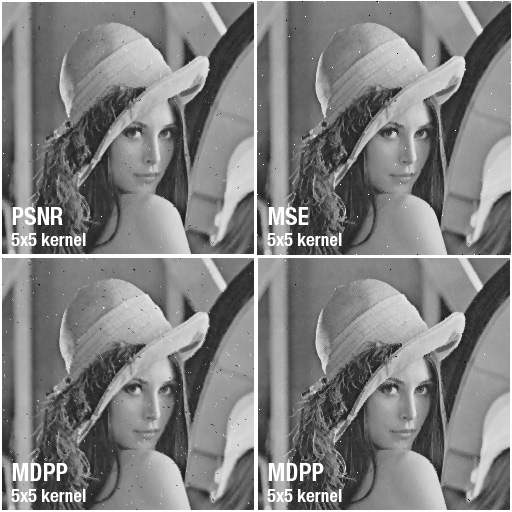
\includegraphics[width=\textwidth]{img/best5.jpg}
			\end{column}
		\end{columns}
			
	\end{frame}	
	
	%% --------------------------
	
		\begin{frame}[t,fragile]
		\frametitle{Sample results - Salt \& Pepper 25\%}
		
		\begin{columns}[onlytextwidth]
			\begin{column}{0.3\textwidth}
				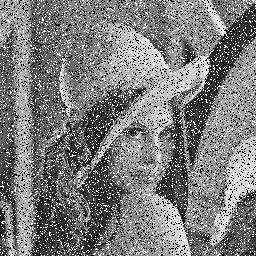
\includegraphics[width=\textwidth]{img/original25.jpg}
				\vspace{3.5mm}
				\scriptsize
				\begin{itemize}
					\item only 5x5 performs well
					\item MDPP: sharpest, but preserves dots
					\item PSNR: blurs
					\item MSE: more blur, tends to average
				\end{itemize}
			\end{column}

			\begin{column}{0.6\textwidth}
				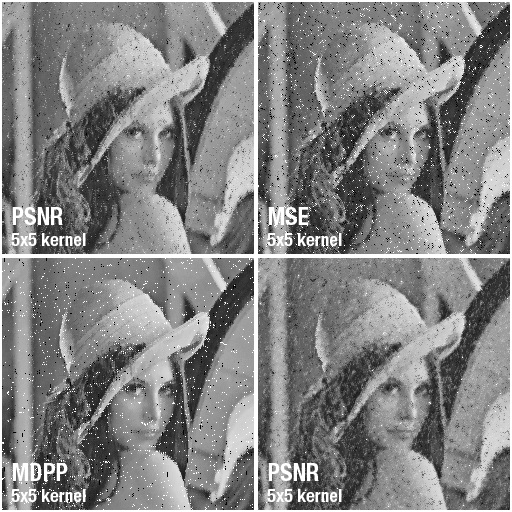
\includegraphics[width=\textwidth]{img/best25.jpg}
			\end{column}
		\end{columns}
			
	\end{frame}	
	
	%% ------------------------------

	\begin{frame}[t,fragile]
	\frametitle{Fitness - MDPP (3x3 kernel, 5\% Salt \& Pepper)}					
	\begin{center}
	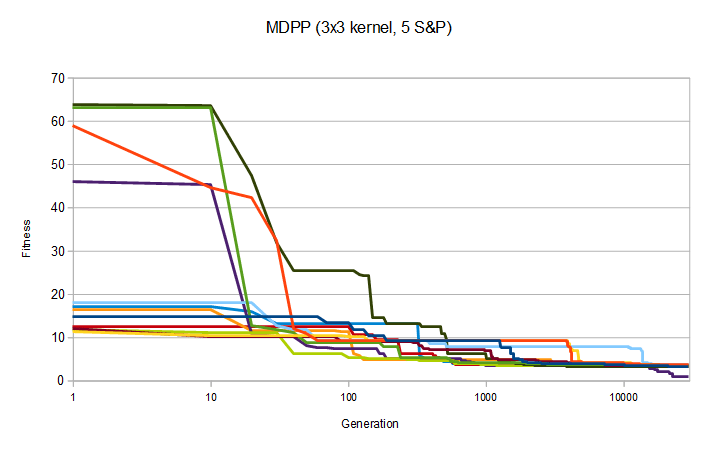
\includegraphics[width=0.9\textwidth]{img/mdpp_3x3_5sp.png}
	
	\end{center}
	\end{frame}
	
		%% ------------------------------

	\begin{frame}[t,fragile]
	\frametitle{Fitness - MDPP (5x5 kernel, 25\% Salt \& Pepper)}					
	\begin{center}
	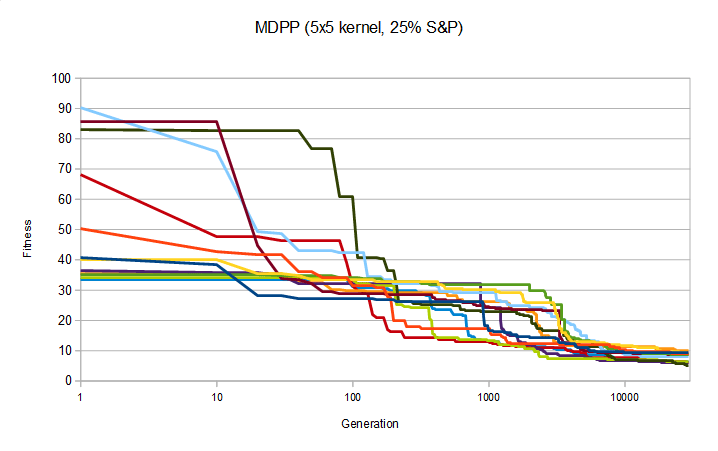
\includegraphics[width=0.9\textwidth]{img/mdpp_5x5_25sp.png}
	
	\end{center}
	\end{frame}
	
		%% ------------------------------

	\begin{frame}[t,fragile]
	\frametitle{Fitness - PSNR (3x3 kernel, 5\% Salt \& Pepper)}					
	\begin{center}
	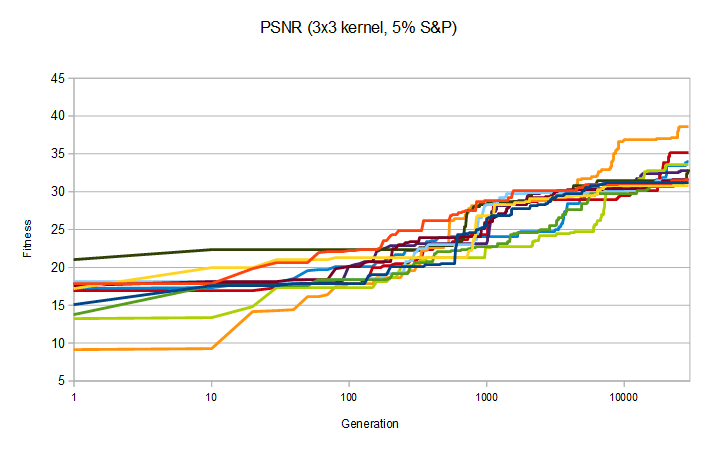
\includegraphics[width=0.9\textwidth]{img/psnr_3x3_5sp.png}
	
	\end{center}
	\end{frame}
	
		%% ------------------------------

	\begin{frame}[t,fragile]
	\frametitle{Fitness - PSNR (5x5 kernel, 25\% Salt \& Pepper)}					
	\begin{center}
	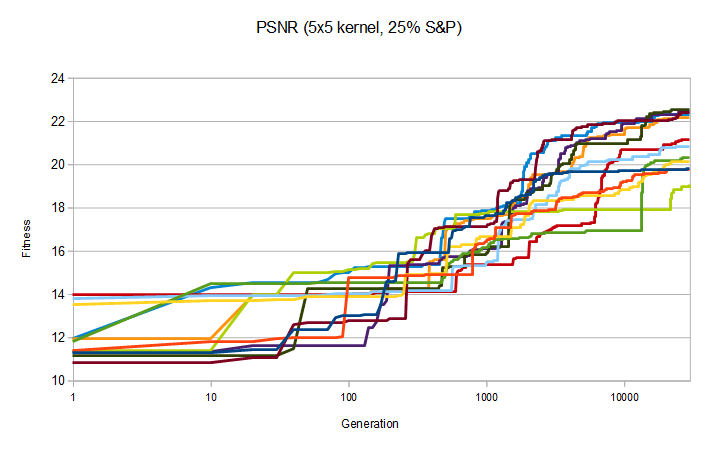
\includegraphics[width=0.9\textwidth]{img/psnr_5x5_25sp.png}
	
	\end{center}
	\end{frame}
	
		%% ------------------------------

	\begin{frame}[t,fragile]
	\frametitle{Fitness - MSE (3x3 kernel, 5\% Salt \& Pepper)}					
	\begin{center}
	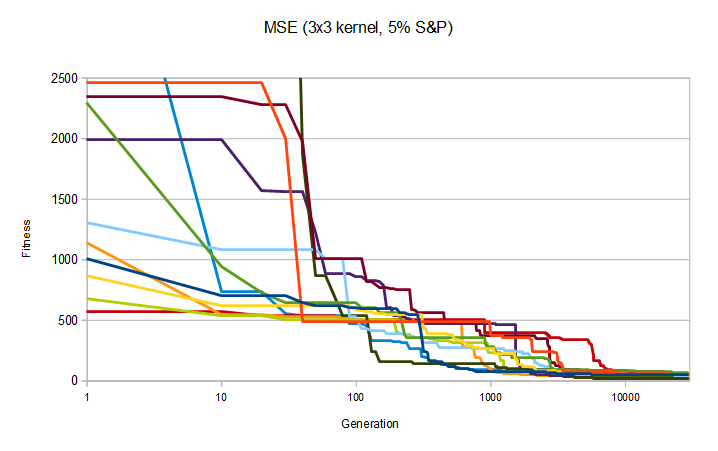
\includegraphics[width=0.9\textwidth]{img/mse_3x3_5sp.png}
	
	\end{center}
	\end{frame}
	
		%% ------------------------------

	\begin{frame}[t,fragile]
	\frametitle{Fitness - MSE (5x5 kernel, 25\% Salt \& Pepper)}					
	\begin{center}
	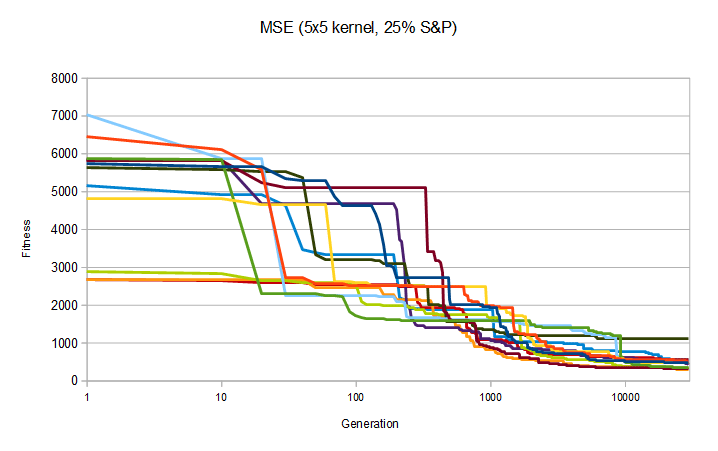
\includegraphics[width=0.9\textwidth]{img/mse_5x5_25sp.png}
	
	\end{center}
	\end{frame}
	
	%% --------------------------
	
	\begin{frame}[t,fragile]
	\frametitle{Summary}	
				
	\begin{itemize}
		\item MDPP and MSE converge faster than PSNR
		\item Less noise converges faster
		\item Size of the kernel doesn't have an effect on convergence
	\end{itemize}				
						
	\end{frame}	
	
		\begin{frame}[t,fragile]
	\frametitle{Fitness - PSNR (100000 generations, 5x5 kernel, 25\% Salt \& Pepper)}					
	\begin{center}
	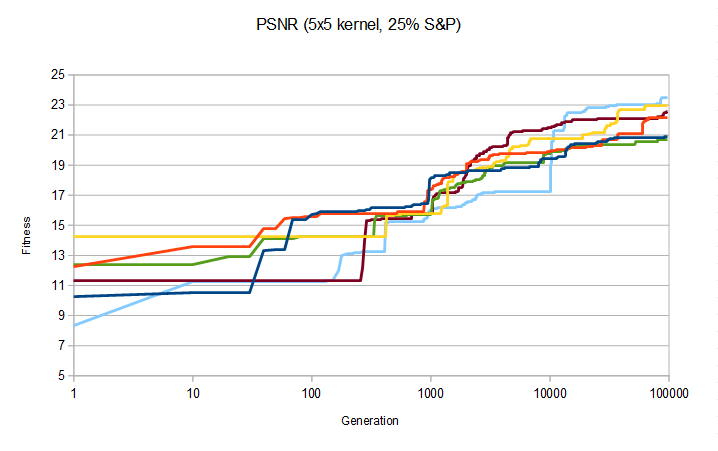
\includegraphics[width=0.7\textwidth]{img/psnr_5x5_25sp_100000.png} \\
	PSNR doesn't seem to converge even after 100000 generations.
	
	\end{center}
	\end{frame}		
	
	%% --------------------------
	
		\begin{frame}[t,fragile]
		\frametitle{Random Impulse Burst Noise 25\% (5x5 kernel)}
		
		\begin{columns}[onlytextwidth]
			\begin{column}{0.3\textwidth}
				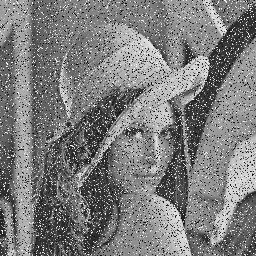
\includegraphics[width=\textwidth]{img/ribn.jpg}
			
			\end{column}

			\begin{column}{0.6\textwidth}
				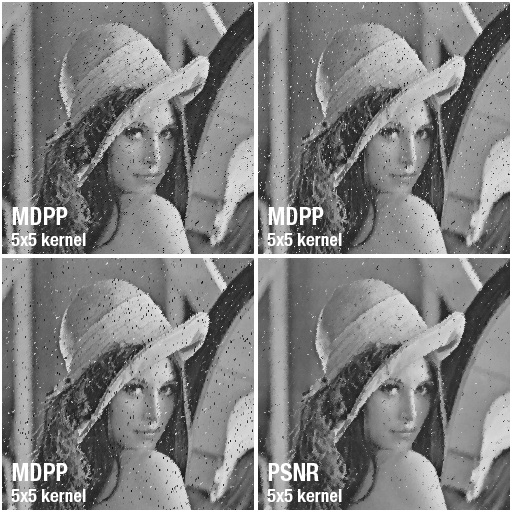
\includegraphics[width=\textwidth]{img/best25_ribn.jpg}
			\end{column}
		\end{columns}
			
	\end{frame}	
	
	%% --------------------------
	
		\begin{frame}[t,fragile]
		\frametitle{Speckle Noise 25\% (5x5 kernel)}
		
		\begin{columns}[onlytextwidth]
			\begin{column}{0.3\textwidth}
				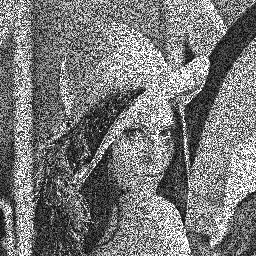
\includegraphics[width=\textwidth]{img/speckle.jpg}				
			\end{column}

			\begin{column}{0.6\textwidth}
				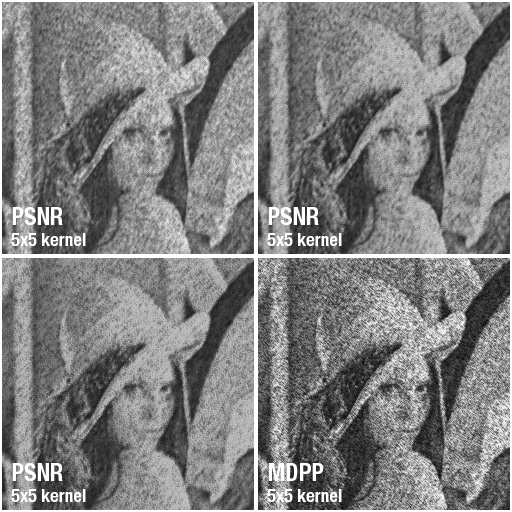
\includegraphics[width=\textwidth]{img/best25_speckle.jpg}
			\end{column}
		\end{columns}
			
	\end{frame}	
	
	

\end{document} 
